%TODO 等的使用
%% TODO 内容问题
%% HACK 粗鄙技巧
%% CODE 代码改进

%TODO——注意事项
%CODE:20160629 每行 80 字符限制,中英文、数字之间加空格

\documentclass[oneside]{book}

%TODO——宏包
%% 页面尺寸
\usepackage{geometry}
	\geometry{
		a4paper,
		left = 2.54 cm, right = 2.54 cm, top = 3.18 cm, bottom = 3.18 cm,
		headheight = 3 cm
	}

%% 设置标题
\usepackage{titlesec}

%% 交叉引用,超链接等
\usepackage[hyperindex]{hyperref}
	\hypersetup{
		%  PDF 书签
		bookmarksopen = true,
		bookmarksopenlevel = 1,
		bookmarksnumbered = true,
		%  PDF 标题作者
		pdftitle = {LaTeX 排版笔记},
		pdfauthor = {曾祥东},
%		%  脚注
%		hyperfootnotes = false,
		%  目录  只引用页码
		linktoc = page,
		%  超链接颜色
		colorlinks,
		linkcolor = {red!60!black},
		citecolor = {green!50!black},
		urlcolor = {blue!63!green}
	}

%% 常规字体选择
%
% 正文字体:Palatino
% 无衬线字体A:Helvetica
% 无衬线字体B:Source Sans Pro
% 等宽字体:Courier
%
% 以下两种方式已弃用:
% Helvetica: \usefont{T1}{phv}{m}{n}
% Courier: \usefont{T1}{pcr}{m}{n}
%
\usepackage[no-math]{fontspec}
	\setmainfont[
		Extension = .otf,
		BoldFont = texgyrepagella-bold,
		ItalicFont = texgyrepagella-italic.otf,
		SlantedFont = texgyrepagella-italic.otf
	]{texgyrepagella-regular}
	\setsansfont[
		Extension = .otf,
		BoldFont = texgyreheros-bold,
		ItalicFont = texgyreheros-italic.otf,
		SlantedFont = texgyreheros-italic
	]{texgyreheros-regular}
	\setmonofont[
		Extension = .otf,
		BoldFont = texgyrecursor-bold,
		ItalicFont = texgyrecursor-italic.otf,
		SlantedFont = texgyrecursor-italic,
		Ligatures = NoCommon
	]{texgyrecursor-regular}
	\newfontfamily{\SourceSans}{Source Sans Pro}
	\newfontfamily{\Songti}{方正书宋_GBK}

%% AMS 数学支持
\usepackage{amsmath}

%% pi 特殊符号
\usepackage{pifont}
	% 正确 √
	\newcommand{\cmark}{\ding{51}}
	% 错误 ×
	\newcommand{\xmark}{\ding{55}}

%% 调用 Unicode OpenType 数学字体
\usepackage{unicode-math}
	\setmathfont[
		math-style = ISO,
		bold-style = ISO
	]{texgyrepagella-math.otf}
% 加粗使用 \symbf{}
% 直立希腊字母:\uppi 等

%% 中文文字处理
\usepackage[UTF8, heading = true]{ctex}
	\ctexset{today = old}
	\pagestyle{empty}

\usepackage{xeCJK}
	\setCJKmainfont[
		BoldFont = 方正黑体_GBK,
		ItalicFont = 方正楷体_GBK,
		SmallCapsFont = 方正书宋_GBK,
		Mapping = fullwidth-stop
	]{方正书宋_GBK}
	\setCJKsansfont[
		BoldFont = 方正黑体_GBK,
		ItalicFont = 方正黑体_GBK,
		Mapping = fullwidth-stop
	]{方正黑体_GBK}
%	\setCJKsansfont[
%		BoldFont = 思源黑体 CN Regular,
%		ItalicFont = 思源黑体 CN Regular,
%		Mapping = fullwidth-stop
%	]{思源黑体 CN Regular}
	\setCJKmonofont[
		BoldFont = 方正仿宋_GBK,
		ItalicFont = 方正楷体_GBK,
		Mapping = fullwidth-stop
	]{方正仿宋_GBK}
	\setCJKfamilyfont{宋体}{方正书宋_GBK}
	\setCJKfamilyfont{楷体}{方正楷体_GBK}
	\setCJKfamilyfont{黑体}{方正黑体_GBK}
	\setCJKfamilyfont{仿宋}{方正仿宋_GBK}

%% 脚注增强版
\usepackage[stable, perpage, bottom]{footmisc}
	% 需要调用 pifont 宏包
	% 衬线加圈阳文数字:\ding{172}~\ding{181} (1~10)
	% 无衬线加圈阳文数字:\ding{192}~\ding{201} (1~10)
	%
	% 脚注不用上标
	%HACK:20160709 见 http://tex.stackexchange.com/q/19844/
	\renewcommand{\thefootnote}{\ding{\numexpr191+\value{footnote} } }
	\makeatletter
	\newlength{\fnBreite}
	\renewcommand{\@makefntext}[1]{%
		\settowidth{\fnBreite}{\footnotesize\@thefnmark.i}
		\protect\footnotesize\upshape%
		\setlength{\@tempdima}{\columnwidth}\addtolength{\@tempdima}{-\fnBreite}%
		\makebox[\fnBreite][l]{\@thefnmark\phantom{  }}%
%		\parbox[t]{\@tempdima}{\everypar{\hspace*{1em}}\hspace*{-1em}\upshape#1}
		}
	\makeatother

%% 颜色
\usepackage[svgnames]{xcolor}

%% 图形
\usepackage{graphicx}

%% 导入 PDF
\usepackage{pdfpages}

%% TeX Logos
\usepackage{hologo}

%% 物理、数学符号
\usepackage{physics}

%% 单位
\usepackage{siunitx}

%% 代码抄录
%\usepackage{shortvrb}
%	\MakeShortVerb |
%CODE:20160908 似乎可以不用
\usepackage{fancyvrb}
	\VerbatimFootnotes

%% 大段代码排版
\usepackage{listings}

%% 彩色、加框环境
\usepackage[listings]{tcolorbox}
	\tcbuselibrary{breakable}
	\tcbset{
		myBoxStyle/.style = {
			% 样式
			colback = Cornsilk, %需要 xcolor 宏包 svgnames 选项
			colframe = gray,
			sharp corners,
			boxrule = 1 pt,
			% 内容边距
			left = 0 cm, right = 0 cm, top = -0.2 cm,
%			各种框型 bottom 设置不同
%			bottom = -0.2 cm,
%			% 文字环绕
%			各种框型设置不同
%			before = {\\ \vspace{-2 ex} \\}, after = {\hspace{\fill}}
			% 分页
			breakable,
			toprule at break = 0 pt, bottomrule at break = 0 pt,
			pad before break = 0.5 ex, pad after break = 3 ex,
		},
		myCodeStyle/.style = {
			listing options = {
				language = tex,
				basicstyle = \ttfamily,
				keywordstyle = \normalsize,
				commentstyle = \color{gray},
				numbers = left,
				numberstyle = \itshape \footnotesize \color{gray},
				breaklines = true,
				escapeinside = {(|}{|)}
			}
		}
	}

%% 定制列表环境
\usepackage{enumitem}
	% 定义带缩进的左对齐格式
	% 前一个参数 2.1 em 确定标签的位置
	% 后一个参数 1.2 em 确定标签与文字的距离
	%HACK:20160709 可能与字体、字号、标签内容有关
	\SetLabelAlign{leftalignwithindent}{\hspace{2.1 em} \makebox[1.2 em][l]{#1}}

%% 定理类环境
%\usepackage[thmmarks, amsmath]{ntheorem}
%	\theoremstyle{plain} %带编号
%%	\theoremheaderfont{\myHeavy}
%	\theorembodyfont{\normalfont}
%%	\theoremsymbol{}
%%	\theoremsymbol{\ensuremath{\triangleleft}}	
%		\newtheorem{_myQuestion}{例}[chapter]
%		\newtheorem{_myAnswer}{答}[chapter]

%% 索引
\usepackage{imakeidx}
	\makeindex[
		name = pkg,
		title = {宏包索引}
	]
	\makeindex[
		name = cmd,
		title = {命令、选项索引}
	]
	\newcommand{\BH}[1]{\hyperpage{#1}}
%	\let \oldindex = \index
%	\renewcommand{\index}[1]{\oldindex{#1|BH}}
	\newcommand{\indexpkg}[1]{\index[pkg]{#1@\pkg{#1}|BH} }
	\newcommand{\indexcmd}[1]{\index[cmd]{#1@\texttt{#1}|BH} }

%% 参考文献
\usepackage[numbers]{natbib}%\raggedleft
%\bibliographystyle{plainnat}
%\bibliographystyle{alpha}
%\bibliographystyle{gbt-7714-2015-numerical}
\bibliographystyle{mybst.new}
% 网址右对齐的实现
%FIXME:20160712 \CTeX logo 在本文档字体下倾斜时重叠
%\providecommand{\url}[1]{\texttt{#1}}
%\providecommand{\urlprefix}{\hspace*{\fill}}

%TODO——环境
%% 问题 Question & Answer (这里的空行用来分段)
% 使用计数器 question,全文统一编号
\newcounter{question}
\setcounter{question}{1}
\renewcommand{\thequestion}{\arabic{question}}
\newenvironment{myQA}[1]
	{%
		{\large \sffamily \noindent \thequestion.~#1}%
		\phantomsection%
		\addcontentsline{toc}{section}{\numberline {\thequestion}#1}
		
	}
	{
		
		\mbox{} \stepcounter{question}
	}

%% 代码框
%FIXME:20160705 不可以使用 tab 键,见 plain.tex 第 18 行
%FIXME:20160714 参数必须要加,否则第一行显示有问题
\newtcblisting{myCode}
	{
		myBoxStyle,
		bottom = -0.2 cm,
		listing only,
		myCodeStyle
	}

%% 水平案例框(左代码,右效果)
% 参数 1:右边栏比例,默认 0.5
% 参数 2:效果的实现
\newtcblisting{myExampleH}[2][0.5]
	{
		myBoxStyle,
		bottom = -0.2 cm,
		listing side comment,
		righthand ratio = #1,
		comment = {#2},
		myCodeStyle
	}

%% 垂直案例框(上代码,下效果)
% 参数 1:效果的实现
\newtcblisting{myExampleV}[1]
{
	myBoxStyle,
	middle = -0.1 cm,
	breakable,
	vfill before first = false,
	listing and comment,
	comment = {#1},
	myCodeStyle
}

%% 供索引使用的抄录环境
%\makeatletter
%\newenvironment{indexverb}{%
%	\def\verbatim@processline{\the\verbatim@line\ }%
%	\def\@verbatim{\the\every@verbatim
%		\obeylines
%		\let\do\@makeother \dospecials
%		\verbatim@font
%	}%
%	\def\endverbatim{\endgroup}%
%	\noindent
%	\verbatim}{\endverbatim}
%\makeatother

%% 定制列表(不编号)
\newenvironment{myItemize}
	{\begin{enumerate} [
		label=\bullet, %标签样式:圆点
		align = leftalignwithindent, %对齐(见上)
		listparindent = 2 em, %条目段落缩进
		leftmargin = 0 pt, %文字左边距
		topsep = 0 pt,
		itemsep = 0 pt,
		parsep = 0 pt
	]}
	{\end{enumerate}}

%TODO——命令
%% 宏包名
\newcommand{\pkg}[1]{{\SourceSans#1}}
%% 文件名
\newcommand{\filename}[1]{\texttt{#1}}
%% 人名超链接
\newcommand{\netname}[1]{\texttt{#1}}
%% 参考文献
\newcommand{\myRef}[1]{\noindent
	{\sc Reference} \raisebox{-0.25 ex}{\ding{43}}
	\quad #1}
%% (La)TeX
% From hologo 宏包, 有修改
%FIXME:20160708 与汉字连用时之前不要加空格
\makeatletter
\DeclareRobustCommand{\LaTeXTeX}{
	(%
	\kern-.1em%
	L%
	\kern-.36em%
	{%
		\sbox\z@ T%
		\vbox to\ht0{%
			\hbox{%
				$\m@th$%
				\csname S@\f@size\endcsname
				\fontsize\sf@size\z@
				\math@fontsfalse
				\selectfont
				A%
			}%
			\vss
		}%
	}%
	\kern-.15em%
	)%
	\kern-.1em%
	\TeX
}
\makeatother
%% 行内命令
% 取消 listings 宏包 \listinline 的 escape 限制
%HACK:20160907 见 http://tex.stackexchange.com/q/43526
\makeatletter
\patchcmd{\lsthk@TextStyle}{\let\lst@DefEsc\@empty}{}{}%
	{\errmessage{failed to patch}}
\makeatother
\newcommand{\code}{\lstinline[
	language = tex,%
	basicstyle = \ttfamily,%
	keywordstyle = \normalsize,%
	commentstyle = \color{gray},%
	escapeinside = {(|}{|)}%
]}
%TODO:20160908 UNICODE 代码
%% Tab 键空格
\newcommand{\tab}{{ {} {} {} }}
%% 命令可选项
\newcommand{\optional}[1]{\textlangle\textit{#1}\textrangle}
%% 空行
\newcommand{\blankline}{\mbox{}}

%TODO——封面
\newcommand{\myCover}{
\includepdf{Cover/Cover.pdf}}
%TODO——标题页
\makeatletter
	\newcommand{\HUGE}{\@setfontsize\Huge{54}{64.8}}
	\newcommand{\myLarge}{\@setfontsize\Huge{30}{36}}
\makeatother
\newcommand{\myTitlePage}{
	\begin{center}
		\vspace*{2 cm}
		{
			\color{Sienna}
			\HUGE
			\LaTeX 排版手记
		}
		
		\vspace{2 cm}
		{
			\color{DarkRed}
			\CJKfamily{楷体} \Huge
			曾祥东
		}
		
		\vspace{12 cm}
		{
			\color{Goldenrod}
			\Huge \scshape \addfontfeature{Numbers=OldStyle}
			\today
		}
	\end{center}
}
%\title{
%	\vspace{-4 cm} \color{Sienna} \Huge \LaTeX 排版笔记
%}
%\author{
%	\CJKfamily{楷体} \color{DarkRed} \Large 曾祥东
%}
%\date{
%	\CJKfamily{楷体} \color{Goldenrod} \Large \today
%}

\begin{document}
	\frontmatter
	
	\myCover
	
	\myTitlePage
	
	\tableofcontents
	
	\mainmatter
	\chapter{文本}
		\begin{myQA}{如何优雅地在科技文献中使用句点?}
	在一般中文文章中,通常使用句号“{\CJKfamily{宋体}。}”。在 Unicode 中,
	它的代码为 \verb|U+3002|。而在科技文献中,为了与一些下标区分,
	经常使用句点“.”(即全角英文句号)
	\footnote{在新的《标点符号用法:GB/T 15834—2011》
		\textsuperscript{\cite{GB/T15834-2011标点符号}} 中,
		这一条被删去了。是否采纳,您看着办。}
	,它的 Unicode 代码为 \verb|U+FF0E|。
	类似符号还有:半角英文句号达到 \verb|U+002E|“.”,
	半角中文句号 \verb|U+FF61|
	\footnote{本文所用字体并不包含该符号,可以脑补一下,
		或者改用微软雅黑等字体来显示。}
	等。这篇文章可以假装是科技文献,因此用了句点。
	
	我们有三种使用句点的方案。
	
	\emph{普青方案}:使用 \pkg{xeCJK} \indexpkg{xeCJK} 宏包的朋友,
	在调用字体时使用
	\verb|Mapping = fullwidth-stop| \indexcmd{Mapping} 选项,
	就可以将正常句号转换成句点。选项 \verb|Mapping = full-stop|
	的作用恰恰相反。
	
	\emph{文青方案}:在导言区添加如下代码即可。此代码第一行将
	“{\CJKfamily{宋体}。}”设置为活动符,并将其定义为命令,从而输出一个句点。
\begin{myCode}
\catcode`\(|{\CJKfamily{宋体}。}|) = \active
\newcommand{(|{\CJKfamily{宋体}。}|)}{.}
\end{myCode}
	\indexcmd{\backslash catcode} \indexcmd{\backslash active}
	
	\emph{二青方案}:利用编辑器全文替换。缺点是这种方式并不优雅。
	
	\myRef{\citet{PKG2016xeCJK}}
\end{myQA}

%HACK:20160708 PDF 标签显示仍为句号,这里改用句点
\begin{myQA}{各种连字符、破折号的区别.}
	在英文中主要有三种:hyphen、en dash 和 em dash。
	
	\begin{myItemize}
		\item  hyphen,-,即连字符,Unicode 代码为 \verb|U+002D|
			\footnote{严格来说,\verb|U+002D| 表示“连字符或减号”。
				Unicode 还单独定义了一个连字符 \verb|U+2010|,
				但是输入不太方便(\verb|\symbol{8208}|)。}
			,用普通键盘就可以直接输入。
		\item en dash,--,即字母“n”宽度的破折号,
			Unicode 代码为 \verb|U+2013|。
			在\LaTeXTeX 中,输入 \verb|--| (即两个 hyphen)可以通过预先
			设定的连字功能得到 en dash。
		\item em dash ,---,想必就是字母“m”宽度的破折号,
			Unicode 代码为 \verb|U+2014|。
			可以通过输入 \verb|---| (即三个 hyphen)来得到。
	\end{myItemize}
	
	\blankline
	
	中文中的连字符也有三种:短横线“{\Songti -}”、一字线“—”和浪纹线“~”。短横线就是上文的 hyphen,而一字线则是 em dash\footnote{观察仔细的话,可以发现它们其实略有差异。这是由于上文的 hyphen 和 em dash 使用了英文字体,而这里的短横线和一字线使用了中文字体。}。剩下的浪纹线,Unicode 代码为 \verb|U+FF5E|。它的输入比较麻烦,毕竟\LaTeXTeX 不是原生支持 Unicode 的。较安全的方法是用 \verb|\symbol{65374}| \indexcmd{\backslash symbol}输入。如果使用 \hologo{XeTeX} 编译,直接在源代码中输入该符号也可以得到。
	
	中文中的破折号是“——”,实际上就是两个连在一起的 em dash。使用中文输入法,一般很容易输入。顺便一说,之前的一字线,可以由破折号删掉一半得到。这实际上是最简单的方法。
	%TODO:20160828 适用范围、参考文献
\end{myQA}

\begin{myQA}{如何在正文中使用上下标?}
	上下标的命令分别是 \verb|\textsuperscript|
	和 \verb|\textsubscript|
	\footnote{在早期版本的 \LaTeX 中,
		使用 \verb|\textsubscript| 命令可能需要调用
		\pkg{fixltx2e} \indexpkg{fixltx2e} 宏包。}
	\indexcmd{\backslash textsuperscript}
	\indexcmd{\backslash textsubscript}。注意要加分组括号,
	否则这两个命令只会对其后的第一个字符起作用。
	
	利用行内公式,也可以实现上下标:
\begin{myExampleV}
{
	\vspace{1 ex}
	
	这是第一个 $^\text{上标}$ 啦啦啦。
	This is another $^\text{supersciprt}$ lalala.
	
	这是第三个$^\text{上标}$啦啦啦。
	This is the fourth$^\text{supersciprt}$lalala.
	
	这是一个$_\text{下标}$。
	This is a $_\text{subscript}$.
}
%% 不要忘记 \usepackage{amsmath}
这是第一个(|\textvisiblespace|)$^\text{上标}$(|\textvisiblespace|)啦啦啦。
This is another(|\textvisiblespace|)$^\text{supersciprt}$(|\textvisiblespace|)lalala.

这是第三个$^\text{上标}$啦啦啦。
This is the fourth$^\text{supersciprt}$lalala.

这是一个$_\text{下标}$。
This is a(|\textvisiblespace|)$_\text{subscript}$.
\end{myExampleV}
	在中文环境中,上下标前后的空格会自动加上,
	无论是不是手动添加。有的时候这会造成麻烦。
	而且这种手段略显猥琐,不推荐使用。
	
	\myRef{\citet{TSE2012superscript,TSE2010subscript}}
\end{myQA}
		
	\chapter{数学与公式}
		\begin{myQA}{如何将实部、虚部用 Re 和 Im 表示?}
	在\LaTeXTeX 中,命令 \verb|\Re| 和 \verb|\Im| 得到的是大写哥特体字母
	$\Re$ \indexcmd{\backslash Re} 和 $\Im$ \indexcmd{\backslash Im}。
	这是高德纳在 \filename{plain.tex} 中定义的。
	
	用下面的命令可以将它们重定义为更常用的格式 $\operatorname{Re}$
	和 $\operatorname{Im}$:
\begin{myCode}
\renewcommand{\Re}{\operatorname{Re}}
\renewcommand{\Im}{\operatorname{Im}}
\end{myCode}
	
	使用 \pkg{physics} \indexpkg{physics} 宏包中的 \verb|\Re| 和 \verb|\Im| 也
	可以达到同样的目的。
	这个宏包还把原来的哥特体保存在了命令 \verb|\real| 和 \verb|\imaginary| 中。
	\indexcmd{\backslash real} \indexcmd{\backslash imaginary}
	
	\myRef{\citet{PKG2012physics}}
\end{myQA}

\begin{myQA}{怎样正确使用微分符号?}
	按照传统,$\dd{x}$、$\dd{\theta}$ 等微元的前后均需要留出一个细空格
	(thin space)的距离。在 \LaTeX 中,细空格用命令 \verb|\,| 表示,
	默认情况下相当于 \SI{3}{mu} 的长度。这个 \si{mu} 表示数学单位,
	一个 \si{mu} 等于 $1/18$ 个 \si{em} 的长度。至于 \si{em},假设你是知道的。
	
	下面是一个例子:
\begin{myExampleV}
{
	\begin{alignat*}{2}
		&\text{错误的:} \quad \iint f(x,y) \mathrm{d}x \mathrm{d}y
		&\quad\quad& \iiint \mathrm{d}r \mathrm{d}\varphi \mathrm{d}\theta \\
		&\text{正确的:} \quad \iint f(x,\,y) \, \mathrm{d}x \, \mathrm{d}y
		&& \iiint \mathrm{d}r \, \mathrm{d}\varphi \, \mathrm{d}\theta
	\end{alignat*}
}
\begin{alignat*}{2}
(|\tab|)&\text{错误的:} \quad
(|\tab|)\iint f(x,y) \mathrm{d}x \mathrm{d}y
(|\tab|)&\quad \quad&
(|\tab|)\iiint \mathrm{d}r \mathrm{d}\varphi \mathrm{d}\theta \\
(|\tab|)&\text{正确的:} \quad
(|\tab|)\iint f(x,\,y) \, \mathrm{d}x \, \mathrm{d}y
(|\tab|)&&
(|\tab|)\iiint \mathrm{d}r \, \mathrm{d}\varphi \, \mathrm{d}\theta
\end{alignat*}
\end{myExampleV}
	但是“\verb|\,|”一多,写起来会很麻烦,而且容易错。惯例,可以新搞一个定义:
\begin{myExampleH}[0.25]
{
	\newcommand{\dif}{\operatorname{d \!}}
	\begin{gather*}
		\iint f(x, \, y) \dif x \dif y \\
		\frac{\dif f}{\dif x} = \sin x \\
		\frac{\dif{^2 g}}{\dif{x^2}} = \cos x
	\end{gather*}
}
%% ----------导言区---------- %%
\DeclareMathOperator{\dif}{d \!}
% 或者 \newcommand{\dif}{\operatorname{d \!}}
%% ----------导言区---------- %%
\begin{gather*}
(|\tab|)\iint f(x, \, y) \dif x \dif y \\
(|\tab|)\frac{\dif f}{\dif x} = \sin x \\
(|\tab|)\frac{\dif{^2 g}}{\dif{x^2}} = \cos x
\end{gather*}
\end{myExampleH}
	这里有两种实现方法。如果用 \verb|\DeclareMathOperator| 的话,
	要注意该声明的代码只能放在导言区。另外这个命令需要
	\pkg{amsmath} \indexpkg{amsmath} 宏包的支持。
	
	这两种方法的原理是类似的。利用数学算子
	(\verb|\DeclareMathOperator| 或 \verb|\operatorname|)
	的命令保证了微分算子前面的间距,又用“\verb|\!|”去掉了它后面的间距。
	同时,这个命令还自动把“$\mathrm{d}$”切换到了直立字体(\verb|\mathrm|)。
	
	如果微分算子“$\mathrm{d}$”后面跟的不是字母,那就不要偷懒,
	该加的分组括号不能少,要不然 bug 会来得出人意料:
\begin{myExampleV}
{
	\newcommand{\dif}{\operatorname{d \!}}
	\begin{alignat*}{4}
		&\text{不好的:} &\quad&
			\dif (\cos x) &\quad \quad&
			\dif \left(\cos x\right) &\quad \quad&
			\dif \left(\frac{\ln x}{x}\right) \\
		&\text{好的:} &&
			\dif{(\cos x)} &&
			\dif{\left(\cos x\right)} &&
			\dif{\left(\frac{\ln x}{x}\right)}
	\end{alignat*}
}
\newcommand{\dif}{\operatorname{d \!}}

\begin{alignat*}{4}
(|\tab|)&\text{不好的:} &\quad&
(|\tab\tab|)\dif (\cos x) &\quad \quad&
(|\tab\tab|)\dif \left(\cos x\right) &\quad \quad&
(|\tab\tab|)\dif \left(\frac{\ln x}{x}\right) \\
(|\tab|)&\text{好的:} &&
(|\tab\tab|)\dif{(\cos x)} &&
(|\tab\tab|)\dif{\left(\cos x\right)} &&
(|\tab\tab|)\dif{\left(\frac{\ln x}{x}\right)}
\end{alignat*}
\end{myExampleV}
	
	普通括号跟在微分算子“$\mathrm{d}$”后面,间距太小,不好看。
	但是如果是定界符括号,间距却又是正常的。所以还是老老实实加上“\verb|{}|”。
	
	\blankline
	
	根据 ISO 80000-2 的要求,微分算子应使用直立的“$\mathrm{d}$”。
	但是,如果你就是任性,非要用斜体的“$d$”,也是可以的。
	把之前代码中的 \verb|d| 用 \verb|\mathnormal{d}| 来代替,
	就可以强制使用斜体(当然前提要求默认数学字体就是倾斜的)。
	
	\blankline
	
	\pkg{physics} \indexpkg{physics} 宏包中定义了 \verb|\differential| 命令
	(简写为 \verb|\dd|),它涵盖了之前我们做的事情,又通过可选参数引入了上标。
	对于圆括号,它还给出了自动处理的解决方案:
\begin{myExampleH}
{
	\begin{equation*}
		\dd x \quad \dd{\theta} \quad \dd[2]{x} \quad
		\dd(\sin \theta) \quad \dd[2](\frac{\ln x}{x})
	\end{equation*}
}
%% ----------导言区---------- %%
\usepackage{physics}
%% ----------导言区---------- %%
\begin{equation*}
(|\tab|)\dd x \quad
(|\tab|)\dd{\theta} \quad
(|\tab|)\dd[2]{x} \quad
(|\tab|)\dd(\sin \theta) \quad
(|\tab|)\dd[2](\frac{\ln x}{x})
\end{equation*}
\end{myExampleH}
	
	另外,这个宏包提供的 \verb|\derivative| 命令(简写为 \verb|\dv|)
	可以类似的手法处理导数:
\begin{myExampleH}
{
\begin{equation*}
\dv{x} \quad \dv{R}{\theta} \quad \dv[n]{f}{x} \quad
\dv{r}(\frac{\ln r}{r})
\end{equation*}
}
%% ----------导言区---------- %%
\usepackage{physics}
%% ----------导言区---------- %%
\begin{equation*}
(|\tab|)\dv{x} \quad
(|\tab|)\dv{R}{\theta} \quad
(|\tab|)\dv[n]{f}{x} \quad
(|\tab|)\dv{r}(\frac{\ln r}{r})
\end{equation*}
\end{myExampleH}
	
	\myRef{\citet{PKG2012physics}}
\end{myQA}

		
	\chapter{字体}
		\begin{myQA}{编译到 \filename{eu1lmr.fd} 时很慢怎么办?}
	据说,只有在 Windows 系统上用 \hologo{XeTeX} 编译时才会出现这种情况。
	\hologo{XeTeX} 会调用系统字体,安装新字体后,需要刷新字体缓存,
	以使 \hologo{XeTeX} 识别新安装的字体。
	可以使用 \verb|fc-cache -f| 命令来重建字体缓存。
	
	关于 \verb|fc-cache| 更多用法,可以输入 \verb|fc-cache --help| 来查看。
	
	在 Mac 上,由于不使用 \filename{fontconfig} 机制,
	因此不会出现该问题。
	
	\myRef{\citet{TSE2015eu1lmr}}
\end{myQA}

\begin{myQA}{cmbright 字体为什么有锯齿?}
	因为
\end{myQA}

\begin{myQA}{如何使用好看的数学字体?}
	\TeX 和 \LaTeX 的默认字体是高老爷子制作的 Computer Modern,
	如图~\ref{Fig:cm_1} 所示。
	%	\begin{equation*}
	%		\int\sin^2 x \,\mathrm{d} x
	%		=\frac{1}{2}x - \frac{1}{4} \sin 2x + C
	%	\end{equation*}
	
	\begin{figure}[h]
		\centering
		\framebox{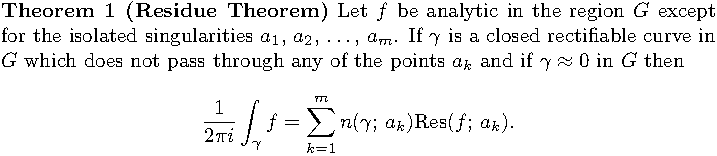
\includegraphics{Examples/cm_1}}
		\caption{Computer Modern 字体示例}
		\label{Fig:cm_1}
	\end{figure}
	
	好看是好看,但是多了也觉得乏味。下面推荐几个字体宏包,给诸位换换口味。
	
	首先是 CM Bright(图~\ref{Fig:cmbright}),这是一个能与
	Computer Modern 相配的无衬线字体,包含在 \pkg{cmbright} 宏包中。
	使用方法是在导言区加上 \verb|\usepackage{cmbright}|。
	
	CM Birght 有一个缺点:少了积分、求和等巨算符。默认采用
	Computer Modern 显示,处女座自是不会满意。不过稍费工夫,
	也有办法改用其他字体(Iwona 之类)。
	%TODO:20160827 需要引用其他问题
	
	\begin{figure}[h]
		\centering
		\framebox{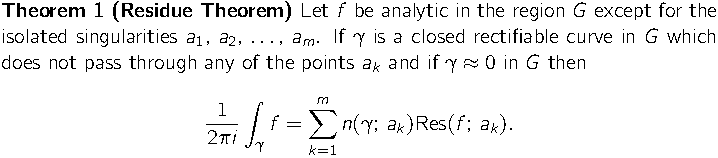
\includegraphics{Examples/cmbright}}
		\caption{CM Bright 字体示例}
		\label{Fig:cmbright}
	\end{figure}
	
	接下来是熟知的 Times 系列。
	
	\begin{figure}[h]
		\centering
		\framebox{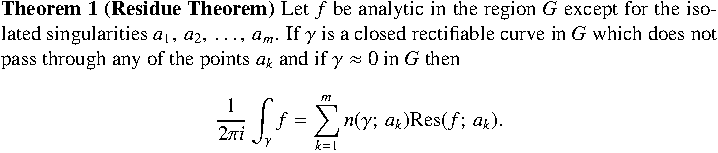
\includegraphics{Examples/txfonts}}
		\caption{Times 字体示例}
		\label{Fig:txfonts}
	\end{figure}
	
	\begin{figure}[h]
		\centering
		\framebox{
\includegraphics{Examples/pxfonts}}
		\caption{Palatino 字体示例}
		\label{Fig:pxfonts}
	\end{figure}
\end{myQA}

\begin{myQA}{如何使用更好看的数学字体?}
\end{myQA}
		
	\chapter{图形}
	\chapter{宏包}
		\begin{myQA}{使用 \pkg{mathdesign} 宏包时
		提示 \filename{texnansi.enc} 无法找到或读取,应该怎么办?}
	\indexpkg{mathdesign}
	典型的编译日志如下(使用 \hologo{pdfLaTeX} 编译):
\begin{myCode}
!pdfTeX error: pdflatex (file texnansi.enc): cannot open encoding file for reading
==> Fatal error occurred, no output PDF file produced!
\end{myCode}
	解决方法是安装 \pkg{ly1} \indexpkg{ly1} 宏包,
	它会提供 \filename{texnansi.enc} 字体编码文件。
	
	\myRef{\citet{TSE2014mathdesign}}
\end{myQA}
		
	\chapter{内核}
		\begin{myQA}{\texttt{\textbackslash newcommand} 和
		\texttt{\textbackslash newcommand*} 有什么区别?}
	\indexcmd{\backslash newcommand} \indexcmd{\backslash newcommand*}
	%
	首先来介绍一点人生经验。
	
	……
	
	用 \code|\newcommand| 来定义命令时,可以使用“长参数”,
	即参数中可以带空行或者 \code|\par| 命令;
	而用 \code|\newcommand*| 来定义命令时,则不可以使用“长参数”。
	
	\myRef{\citet{TSE2012newcommand}}
\end{myQA}
	\backmatter
	{
		\nocite{*}
		\small
		\bibliography{Reference}
	}
	\printindex[pkg]
	\printindex[cmd]
\end{document}